%iffalse
\let\negmedspace\undefined
\let\negthickspace\undefined
\documentclass[journal,12pt,onecolumn]{IEEEtran}
\usepackage{cite}
\usepackage{amsmath,amssymb,amsfonts,amsthm}
\usepackage{algorithmic}
\usepackage{multicol}
\usepackage{graphicx}
\usepackage{textcomp}
\usepackage{xcolor}
\usepackage{txfonts}
\usepackage{listings}
\usepackage{enumitem}
\usepackage{mathtools}
\usepackage{gensymb}
\usepackage{comment}
\usepackage[breaklinks=true]{hyperref}
\usepackage{tkz-euclide} 
\usepackage{listings}
\usepackage{gvv}                                        
%\def\inputGnumericTable{}                                 
\usepackage[latin1]{inputenc}                                
\usepackage{color}                                            
\usepackage{array}                                            
\usepackage{longtable}                                       
\usepackage{calc}                                             
\usepackage{multirow}                                         
\usepackage{hhline}                                           
\usepackage{ifthen}                                           
\usepackage{lscape}
\usepackage{tabularx}
\usepackage{array}
\usepackage{float}
\newtheorem{theorem}{Theorem}[section]
\newtheorem{problem}{Problem}
\newtheorem{proposition}{Proposition}[section]
\newtheorem{lemma}{Lemma}[section]
\newtheorem{corollary}[theorem]{Corollary}
\newtheorem{example}{Example}[section]
\newtheorem{definition}[problem]{Definition}
\newcommand{\BEQA}{\begin{eqnarray}}
\newcommand{\EEQA}{\end{eqnarray}}
\newcommand{\define}{\stackrel{\triangle}{=}}
\theoremstyle{remark}
\newtheorem{rem}{Remark}

% Marks the beginning of the document
\begin{document}
\bibliographystyle{IEEEtran}
\vspace{3cm}

\title{\textbf{NCERT 9.4.3}}
\author{EE24BTECH11032- John Bobby}
\maketitle
\bigskip
\textbf{Question:} Find the solution for the differential equation $\frac{dy}{dx}+y=1$\\
\section{Mathematical Approach} 
\begin{align*}
    \frac{dy}{dx}=1-y\\
\end{align*}
On rearranging the terms,
\begin{align*}
    \frac{dy}{1-y}&=dx\\
    \int \frac{dy}{1-y}&=\int dx\\
    -\log{\abs{y-1}}+c_1&=x+c_2
\end{align*}
On simplification 
\begin{align*}
    -\log{\abs{y-1}}=x+c\\
    \abs{y-1}=\pm e^{-x}\\
    y=1\pm e^{-x}\\
\end{align*}
For the numerical approach we are assuming that the function passes through origin\\
Thus is the function $y$ is,
\begin{align*}
    y=1-e^{-x}
\end{align*}
\section{Numerical Approach}
\begin{align*}
\frac{dy}{dx}=\lim_{h \rightarrow 0} \frac{y\brak{x+h}-y\brak{x}}{h}
\end{align*}
If $h$ is sufficiently small,\\
\begin{align*}
    y\brak{x+h}-y\brak{x}=h\frac{dy}{dx}\\
    y\brak{x+h}=y\brak{x}+h\frac{dy}{dx}
\end{align*}
Thus the value of $y\brak{x+h}$ can be predicted if we know the value of the derivative at that point\\
For this question 
\begin{enumerate}
    \item The interval $\sbrak{0,100}$ is divided  into $1000$ equal parts each of width $0.1$units
    \item On starting from a known point $\brak{x,y}$ the value for $y\brak{x+0.1}$ is calculated. This procedure is repeated until the value of $x$ reaches 100.
    \item Knowing all the $y$ values for the equally spaced $x$ values in interval, the solution plot can be plotted.
\end{enumerate}
\newpage
The plot is given below\\
\begin{figure}[h!]
    \centering
    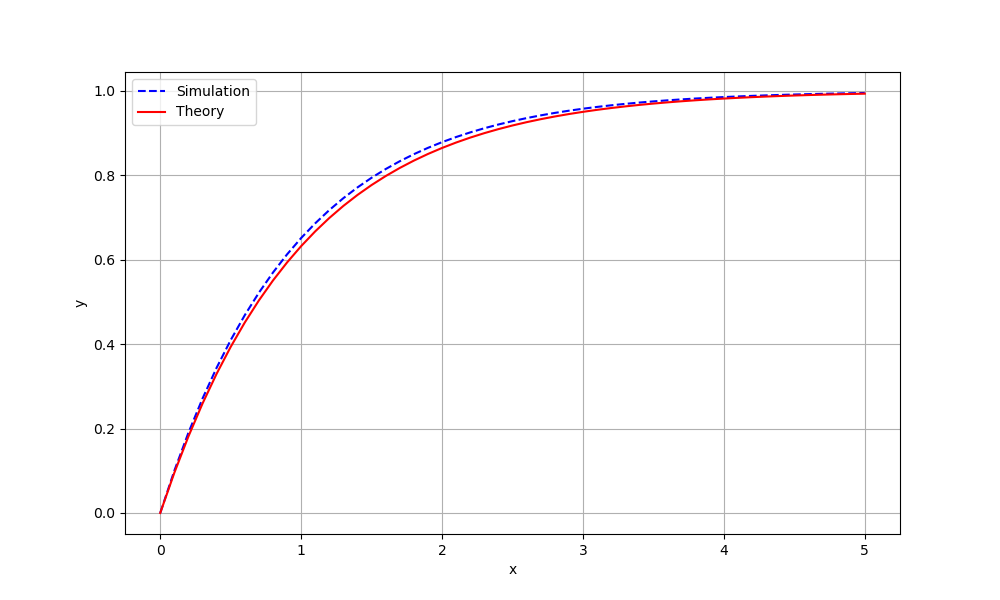
\includegraphics[width=0.7\columnwidth]{figs/Q1.png}
    \label{stemplot}
\end{figure}






\end{document}
